After completion of the exercise routine, we presented each participant with two types of feedback. First, a holistic one (see Figure 2), which consisted of two percentages summarizing how the participant performed relative to our expert benchmark: rate percentage alone and rate percentage after accounting for form.  Second, a granular one comprising a detailed output of our data processing, including graphs and rates for each exercise. 
Figure 3 shows example output of the granular feedback for squat jumps: it displays the average rate per second as well as a graph 
showing how high the participant jumped over the course of the exercise. 
(Notice that the participant was jumping relatively higher at the beginning of the set than at the end, perhaps due to a loss of stamina.)
%%%%%%%%%%%%%%%%%%%%%%%%%%%%%%%%
\begin{figure}[h!]
	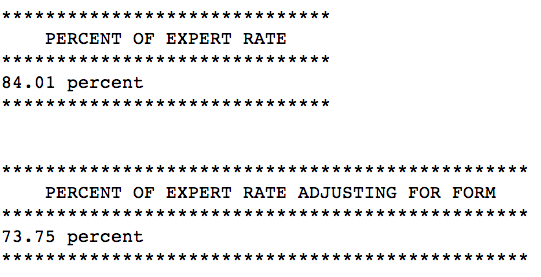
\includegraphics[width=0.5\textwidth]{images/holistic}
\caption{Feedback Design 1: Holistic}
\end{figure}
%%%%%%%%%%%%%%%%%%%%%%%%%%%%%%%%
\begin{figure}[h!]
	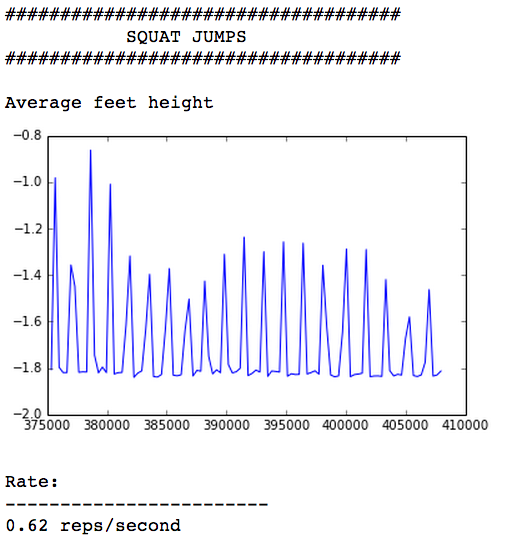
\includegraphics[width=0.5\textwidth]{images/granular}
\caption{Feedback Design 2: Granular}
\end{figure}
%%%%%%%%%%%%%%%%%%%%%%%%%%%%%%%%
We then asked which type of feedback the participant would find most helpful as a means of tracking progress and improvement over time, and recorded their response. 
